%\documentclass[12pt]{article}
%\usepackage[margin=1 in, head=0.9 in]{geometry}
%\usepackage{fancyhdr}
%\usepackage{listings}
%\usepackage{caption}
%\usepackage{color}
%\usepackage{xcolor}
%\usepackage{caption, apacite}
%\DeclareCaptionFont{white}{\color{white}}
%\DeclareCaptionFormat{listing}{\colorbox{gray}{\parbox{\textwidth}{#1#2#3}}}
%\captionsetup[lstlisting]{format=listing,labelfont=white,textfont=white}
%\usepackage{graphicx}
%\usepackage{amsmath, amssymb, amsthm}
%\usepackage[all,cmtip]{xy}
%\pagestyle{fancy}
\input{/home/dmitry/Work/Research/thesis/FINALE/settings.tex}

\begin{document}

\title{Gravity wave scattering by large scale sea bottom features}
\maketitle

\section{Abstract}
Oceanic gravity waves fundamentally contribute to redistribution of mechanical energy in the world ocean. Energy transfer from wave generation sites to dissipation regions are controlled by the physics of gravity waves. The energy transfer occurs not only in the lateral direction but also by conversion into vertical movements such as internal waves. For surface and interior fluid motions, interaction with the sea bottom irregularities can alter gravity wave energy pathways. That is energy can be reflected and scattered both in different directions and into propagation modes. My PhD project addresses wave scattering and reflection by sea bottom features in two important cases: a tsunami wave scattered from a prominent sea mount and reflection of a semidiurnal internal tide from a continental slope.\\
Evidently, bottom bathymetry determines local wave behaviour both for barotropic and baroclinic modes. The gravity wave scattering and excitation of subsidiary wave patterns controls energy pathways on the world ocean scales. This thesis intends to investigate physical aspects of wave energy scattering, mode conversion over topographic features and variability in these process.\\
Interactions of tsunami waves with seafloor topography can delay and redirect the energy flux, \textit{creating amplified waves with long periods}. During the March 2011 tsunami event in Japan tide stations in Northern and Central California recorded large waves, while much smaller waves were observed in Washington and in the southern California. This correlated with a ray of high energy originating from the distant scattering from Emperor seamount chain and more specifically from Koko Guyot. This underwater feature focuses energy into tight beams. This investigation shows that guoyt's shape is responsible for the observed signals. The 2011 tsunami event is compared with a case of Kuril tsunami of 2006. The comparative analysis emphasis strong correlation between frequency of incident tsunami wave component, its propagation direction and the observed signal at Northern California.\\
The energy can be distributed not only by surface expression of the sea but also in the ocean's interior. Internal tides originate as surface tide encounters steep topographic feature. At such location the energy would drain into perturbations of isopycnals that further can travel hundreds of  leagues without any significant loss of energy. In the second part of my thesis origination, propagation and dissipation of the internal tidal beam is investigated on the example of Tasman Sea. 
A global internal tide model, satellite altimetry measurements and in situ observations indicate that a ridge south of New Zealand is a site for the generation of the strong tidal beam that is directed towards the Tasman Shelf break. The low mode internal wave beam undergoes scattering from topography, which transfers energy to shorter length scales. Thus, understanding of local energy processes will lead to a more detailed picture of tidal energy dissipation.\\
\textbf{CONCLUSIONS}

\section*{Questions to answer:}
\begin{itemize}
\item Why did you work on this problem?\\
My interest in this problem spurred from complexity of wave-topography interactions. As wave encounters considerable inhomogeneity in the ocean bottom its behavior rapidly changes with its initial energy being redistributed into other forms of propagation. For example, for many years it was known trapping of wave energy at bottom discontinuity. This is a classical problem leading to an idea that the ocean waves will be redistributing energy in different locations, enlightening some regions of the ocean or creating shadow zones. My thesis considers such two problems. First is about tsunami wave that focus their energy and thus, creating amplified signals at distant locations along coastlines. For the second problem it is taken internal tidal beam that hits continental margin with consequent energy deposition. My primary question was to analyze numerical experiments and describe physical mechanisms behind in order to quantify the scattering problem.\\

\item What did you find out?\\
Tsunami wave as it encounters submerged mountain will excite spatial modes that has quite tight structure. More appropriatly to call them tsunami beams. They will have frequency dependence, only specific periods and under specific incident angle will generate the tsunami beams. This further led to description of two tsunami events that had distinct signature along the west coast of the US that is supported by sea level gauge observations. It appears that seamounts can focus energy under distinct conditions, which would help in future analysis of tsunami events.\\
On the other hand, internal tides in Tasman Sea show variability and hence, their scattering on the continental slope will have time variable character. But this turns out to be dependent not only local conditions around Tasmania, but also generation process occurring at Macquarie Ridge. Putting everything together has shown that the energy deposition will vary. This is well known result, but in my work I have investigated and described the processes beneath such that position of large scale circulation can change the incidence of the beam decreasing its dissipation on the slope, but further offshore conditions can additionally refract the beam. When the beam impinges the slope it can additionally excite some transport phenomena - slope mode which shuffles energy around the slope. In overall, my work proposed ideas and methods how such variable behavior can be understood and predicted.

\item How did you tackle it?\\
These problems were addressed by analysis of energy flux budgets. This quantity is useful in analysis of scattering and reflection problems since energy conservation is one of the fundamental principles. Calculating energy flux and carrying out developed in my thesis method for directional decomposition with additional analysis of conversion rates for internal tides led to understanding how energy is partitioned between different modes of both horizontal and vertical propagation. Than it was developed theoretical framework to generalize the considered here problems and to study parameter space.
\end{itemize}

\section{Introduction}
Gravity waves are ubiquotous feature of the World Ocean. The fundamental importance of the linear gravity waves is their ability to transfer momentum over large length scales. The energy pathways of propagating gravity waves can be altered in a result of interaction with large scale sea bottom features such as submarine seamountains, trenches and continental shelves. These processes appreciably shape wave propagation, and thus, leading to variation in localized energy budgets. In this work two geophysically important cases are considered. Two examples of energy scattering will be considered in this thesis work.\\
The first deals with tsunami waves (\textbf{HERE IT GOES LONG INTRODUCTION to TSUNAMI WAVE: IMPORTANCE, WHERE IT OCCURS, WHAT IT CAUSES, SECTION?})\\
What is missing? References. More generalization? Decay? Murty, Rabinovich, Kowalik, that Greek lady.
Tsunami waves are transient waves occurring owing to its generation earthquakes along deep ocean trenches. Rapid uplift of sea bottom creates a hump water that further freely propagates away from the trench in deep ocean. During their transoceanic propagation these waves encounter numerous large scale ocean bottom roughness such as seamount chains and submarine plateaus. All of these obstacles can redirect tsunami propagation because of rapid change in ocean depth. This phenomena is well known as wave refraction in coastal oceanography.\\
For the US it is of most importance understanding how tsunami waves are transformed when their origination lays along Japan-Kuril trench (Figure 1 map. There one of the most disruptive and powerful events in the recorded history occurred. For example, tsunami event happened near Japan on March 12, 2011 created a devasting wave that caused huge along shore run ups in Japan, the wave crossed the Northern Pacific Ocean and caused severe economical losses to the West Coast. In this example it is emphasized that interaction with prolonged chain of seamounts known Emperor Seamount chain has created additional conditions for relatively directive and focused signal on the West Coast.\\
Several previous studies have identified that the primary source of scattering of tsunami waves in Pacific Ocean is Koko Guoyt. Here the secondary waves originate from interaction with steep seamount. Later secondary waves form a distinctive beam which has its final destination towards Mendocino Escarpment where additional focusing occurs bringing amplified waves to Crescent City, CA. In such scenario it is notable that observations suggest arrival of the secondary waves long after the main tsunami wave arrival occurs. Hence, developing understanding of mechanisms behind generation of the scattered tsunami waves have important forecasting consequences. This work is developing a description for such mechanism.\\

\begin{figure}
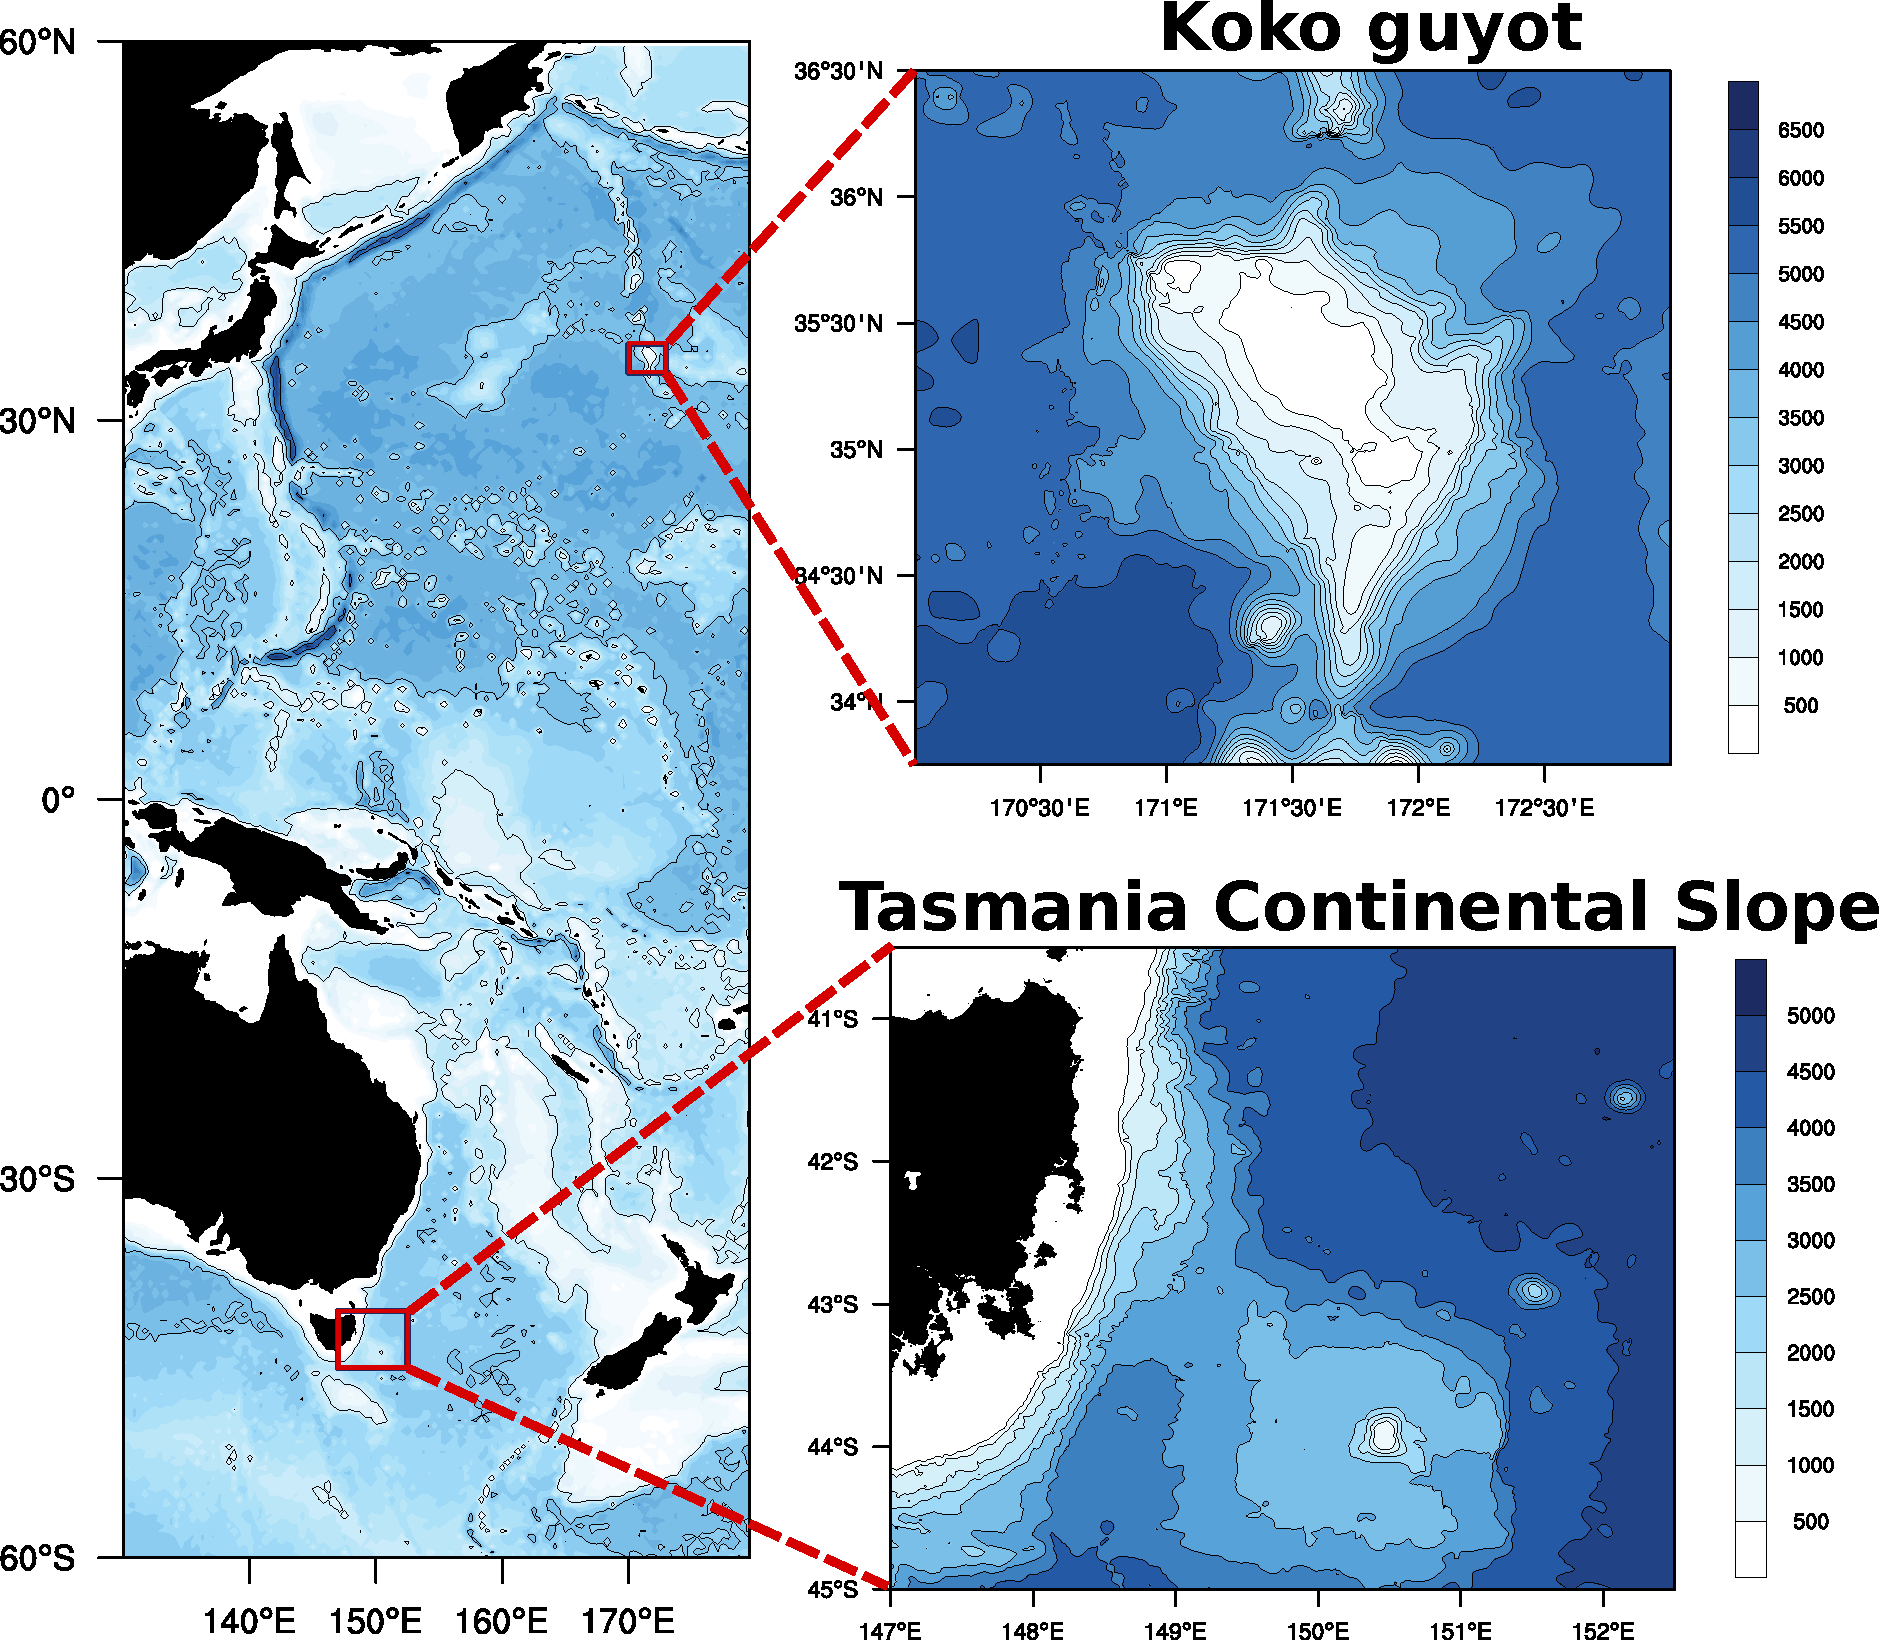
\includegraphics[scale=0.5]{../figures/map_w_places.pdf}
\caption{The map of the Pacific Ocean with outlined regions.}
\end{figure}

Tsunami waves propagate 1000s of kilometers without almost any dissipation of their energy. At their arrival at distant locations such as shorelines the carried mechanical energy leads to devasting events: strong currents and high runups.\\
(\textbf{HERE IT GOES LONG INTRODUCTION to INTERNAL TIDES, GENERATION, GLOBAL SCALE, IMPORTANCE, SECTION?})\\
Another example of energy transfer over long distances is a baroclinic waves of tidal frequencies (internal tides). Their origin usually occurs at long ridge chains. As they cross ocean basins they as well preserve much of their initial energy content which further lead to deposition of the energy.\\

\subsection{Energy conservation and energy flux}
I take shallow gravity framework that works well for tsunami propagation in deep ocean. For internal tides the Boussinesq equations can be transformed into Laplace tidal equations after vertical eigenmode decomposition.\\

Energy flux appears as...\\
Nonlinearity\\

\subsection{Formulation of scattering problem}
Generally speaking, wave scattering happens due to inconsistency of boundary conditions. This can be expressed as the following equation.

\newpage
\section{TO DO}
\begin{itemize}
\item In my writing here I need to write down energy conservation equation. It must be done super careful. Ref: Wunsch, Ferrari; Nekrasov; 
\item Definition of energy flux since it is corner stone for the whole work. Ref: Kowalik papers; Nash, Kelly

\end{itemize}

\bibliographystyle{apacite}
\bibliography{/home/dmitry/Bibtex_lib/}

\end{document}